\documentclass[a4paper, 12pt]{article}

\usepackage{mathtext}
\usepackage[T2A]{fontenc}
\usepackage[utf8]{inputenc}
\usepackage[russian]{babel}

\usepackage{amsmath}
\usepackage{titlesec}
\usepackage{scrextend}
\usepackage{graphicx}
\usepackage{tikz}
\usetikzlibrary{shapes.misc}
\usepackage{pdflscape}

\DeclareSymbolFont{T2Aletters}{T2A}{cmr}{m}{it}
\graphicspath{ {./images/} }

% Установки для отрисовки решеток кодера
\tikzstyle{lightedge}=[dashed]
\tikzstyle{mainedge}=[solid]
\tikzstyle{activeedge}=[green, very thick]
\tikzstyle{inputBit}=[rectangle,fill=red, text=white]
\tikzstyle{outputBit}=[rectangle,fill=blue, text=white]
\tikzstyle{pointer}=[orange,->,dashed]
\tikzstyle{highlight}=[circle,fill=blue,text=white,scale=0.7]

\newcounter{ctra}
\newcommand{\trellisEdges}[2]{
  \setcounter{ctra}{#2}
  \pgfmathtruncatemacro{\xplusone}{#1 + 1}
  \ifodd\value{ctra}
      \draw[mainedge] (s#1#2) -- (s\xplusone2);
  \else
      \draw[mainedge] (s#1#2) -- (s\xplusone0);
  \fi
  \ifodd\value{ctra}
      \draw[lightedge] (s#1#2) -- (s\xplusone3);
  \else
      \draw[lightedge] (s#1#2) -- (s\xplusone1);
  \fi
}

% #1=x; #2=y; #3=In; #4=Out
\newcommand{\trellisInOut}[4]{
  \node[inputBit] (in#1) at (#1+0.5,4) {#3};
  \node[outputBit] (out#1) at (#1+0.5,5) {#4};
  \draw[pointer] (in#1) -- (#1+0.5,#2);
}

% #1=x; #2=y; #3=In
\newcommand{\trellisIn}[2]{
  \node[outputBit] (in#1) at (#1+0.5,4) {#2};
}


\author{Анатолий Копыл}
\title{Курсовая работа}

\begin{document}

\section{Исходные данные}
\[ m=41 \]
\begin{center}
  \begin{tabular}{ | p{5cm} | p{5cm} | p{5cm} | } 
    \hline
    Предельные уровни аналогового сигнала \(a_{min}\), \(a_{max}\) (В) & \(a_{max}=25,6\) В;\newline\(a_{min}=-25,6\) В & Внести свои данные \\
    \hline
    Верхняя частота спектра аналогового сигнала \(f_В\) & \(f_В =(1+m\cdot 10^{-2})\cdot 10^4\) & \(f_В =14100\) \\ 
    \hline
    Заданный уровень квантования & \(j=500-3\cdot m\) & 377 \\
    \hline
    Спектральная плотность мощности флуктуационной помехи & 41 & \(N_0=2,3\cdot 10^{-7}\, В^2/Гц\)\\
    \hline
    q - номер тактового интервала ошибки & \(q=m\mod{3}+1\) & \(q=3\)\\
    \hline
    Вид модуляции & КАМ-16 & \\
    \hline
  \end{tabular}
\end{center}

\section{Аналого-цифровой преобразователь}
\[ \Delta t \leq \frac{1}{2f_B}=\frac1 {2\cdot 14100} = 3,546\cdot 10^{-5}\, с \]
\[ f_d=\frac{1}{\Delta t}\geq 2f_B=\frac{1}{3,546\cdot 10^{-5}}=28200 \]
\[ 377_{10}=101111001_2 \]
\[ k=9;\, L=2^9 = 512 \]

\section{Кодер}
\begin{center}
  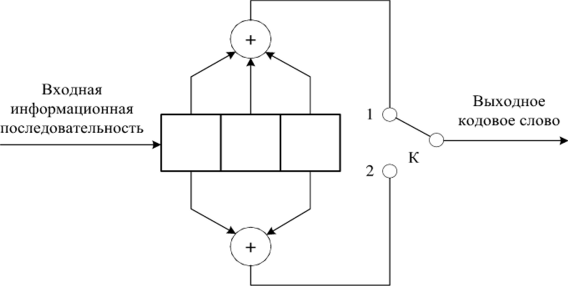
\includegraphics[scale=0.8]{coder}

  \begin{tabular}{ | c | c | c | c | c | c | c | c | c | c | }
    \hline
    Входной сигнал &1&0&1&1&1&1&0&0&1\\
    \hline
    Выходной сигнал &11&10&00&01&10&10&01&11&11\\
    \hline
  \end{tabular}
\end{center}

\subsection{Решетка кодера}
\begin{figure}[H]
  \begin{tikzpicture}[x=1.2cm, y=-1cm]
    \node at (-0.5,0) [left] {$s_1=00$};
    \node at (-0.5,1) [left] {$s_2=10$};
    \node at (-0.5,2) [left] {$s_3=01$};
    \node at (-0.5,3) [left] {$s_4=11$};

    % Nodes
    \foreach \x in {0,...,9} {
      \node at (\x,-.7) {$\x$};
      \foreach \y in {0,...,3} {
        \node (s\x\y) at (\x,\y) [circle,fill=black,scale=0.7] {};
      }
    }

    % Edges
    \trellisEdges{0}{0}
    \trellisEdges{1}{0}
    \trellisEdges{1}{1}
    \foreach \x in {2,...,8} {
      \foreach \y in {0,...,3} {
        \trellisEdges{\x}{\y}
      }
    }

    % Inputs and Outputs
    \node at (-0.5,4) [left] {Входной бит};
    \node at (-0.5,5) [left] {Результат};

    \trellisInOut{0}{0.5}{1}{11}
    \trellisInOut{1}{1.5}{0}{10}
    \trellisInOut{2}{1.5}{1}{00}
    \trellisInOut{3}{2}{1}{01}
    \trellisInOut{4}{3}{1}{10}
    \trellisInOut{5}{3}{1}{10}
    \trellisInOut{6}{2.5}{0}{01}
    \trellisInOut{7}{1}{0}{11}
    \trellisInOut{8}{0.5}{1}{11}
  \end{tikzpicture}

  \caption{Решетка кодера} \label{fig:coder}
\end{figure}

Длительность двоичного символа \(T_В\) на выходе кодера:
\[T_В=\frac{\Delta t}{2k}=\frac{3,546\cdot 10^{-5}}{2\cdot 9}=
1,97\cdot 10^{-6}\,с\]

\section{Декодер}
По каналу передавался код \(\overline{u}=11 10 00 01 10 10 01 11 11\).
Ошибка произошла на тактовом интервале \(q=3\).
Таким образом, на вход декодера поступает последовательность 
\(\overline{Z}=11 \dot{0}0 00 01 10 10 01 11 11\). Точкой обозначен ошибочно принятый символ.

\subsection{Диаграмма декодера}
\begin{figure}
  \begin{tikzpicture}[x=1.2cm, y=-1cm]

    \node at (-0.5,0) [left] {$s_1=00$};
    \node at (-0.5,1) [left] {$s_2=10$};
    \node at (-0.5,2) [left] {$s_3=01$};
    \node at (-0.5,3) [left] {$s_4=11$};

    % Nodes
    \foreach \x in {0,...,9} {
      \node at (\x,-.7) {$\x$};
      \foreach \y in {0,...,3} {
        \node (s\x\y) at (\x,\y) [circle,fill=black,scale=0.7] {};
      }
    }

    \node at (0,0) [highlight] {};
    \node at (1,0) [highlight,label=left:{$2$}] {};
    \node at (1,1) [highlight,label=left:{$0$}] {};

    \node at (2,0) [highlight,label=left:{$0$}] {};
    \node at (2,1) [highlight,label=left:{$2$}] {};
    \node at (2,2) [highlight,label=left:{$1$}] {};
    \node at (2,3) [highlight,label=left:{$1$}] {};

    \node at (3,0) [highlight,label=left:{$\frac{0}{2}$}] {};
    \node at (3,1) [highlight,label=left:{$\frac{2}{0}$}] {};
    \node at (3,2) [highlight,label=left:{$\frac{1}{1}$}] {};
    \node at (3,3) [highlight,label=left:{$\frac{1}{1}$}] {};

    \node at (4,0) [highlight,label=left:{$\frac{1}{1}$}] {};
    \node at (4,1) [highlight,label=left:{$\frac{1}{1}$}] {};
    \node at (4,2) [highlight,label=left:{$\frac{2}{0}$}] {};
    \node at (4,3) [highlight,label=left:{$\frac{0}{2}$}] {};

    \node at (5,0) [highlight,label=left:{$\frac{1}{1}$}] {};
    \node at (5,1) [highlight,label=left:{$\frac{1}{1}$}] {};
    \node at (5,2) [highlight,label=left:{$\frac{0}{2}$}] {};
    \node at (5,3) [highlight,label=left:{$\frac{2}{0}$}] {};

    \node at (6,0) [highlight,label=left:{$\frac{1}{1}$}] {};
    \node at (6,1) [highlight,label=left:{$\frac{1}{1}$}] {};
    \node at (6,2) [highlight,label=left:{$\frac{0}{2}$}] {};
    \node at (6,3) [highlight,label=left:{$\frac{2}{0}$}] {};

    \node at (7,0) [highlight,label=left:{$\frac{1}{1}$}] {};
    \node at (7,1) [highlight,label=left:{$\frac{1}{1}$}] {};
    \node at (7,2) [highlight,label=left:{$\frac{2}{0}$}] {};
    \node at (7,3) [highlight,label=left:{$\frac{0}{2}$}] {};

    \node at (8,0) [highlight,label=left:{$\frac{2}{0}$}] {};
    \node at (8,1) [highlight,label=left:{$\frac{0}{2}$}] {};
    \node at (8,2) [highlight,label=left:{$\frac{1}{1}$}] {};
    \node at (8,3) [highlight,label=left:{$\frac{1}{1}$}] {};

    \node at (9,0) [highlight,label=left:{$\frac{2}{0}$}] {};
    \node at (9,1) [highlight,label=left:{$\frac{0}{2}$}] {};
    \node at (9,2) [highlight,label=left:{$\frac{1}{1}$}] {};
    \node at (9,3) [highlight,label=left:{$\frac{1}{1}$}] {};

    % Edges
    \trellisEdges{0}{0}
    \trellisEdges{1}{0}
    \trellisEdges{1}{1}
    \foreach \x in {2,...,8} {
      \foreach \y in {0,...,3} {
        \trellisEdges{\x}{\y}
      }
    }

    % Inputs
    \node at (-0.5,4) [left, align=right] {Входная\\пара};

    \trellisIn{0}{11}
    \trellisIn{1}{00}
    \trellisIn{2}{00}
    \trellisIn{3}{01}
    \trellisIn{4}{10}
    \trellisIn{5}{10}
    \trellisIn{6}{01}
    \trellisIn{7}{11}
    \trellisIn{8}{11}
  \end{tikzpicture}

  \caption{Решетка декодера} \label{fig:decoder}
\end{figure}

\begin{figure}
  \begin{tikzpicture}[x=2cm, y=-1cm]

    \node at (-0.5,0) [left] {$s_1=00$};
    \node at (-0.5,1) [left] {$s_2=10$};
    \node at (-0.5,2) [left] {$s_3=01$};
    \node at (-0.5,3) [left] {$s_4=11$};

    % Nodes
    \foreach \x in {0,...,3} {
      \node at (\x,-.7) {$\x$};
      \foreach \y in {0,...,3} {
        \node (s\x\y) at (\x,\y) [circle,fill=black,scale=0.7] {};
      }
    }

    % Edges
    \trellisEdges{0}{0}
    \trellisEdges{1}{0}
    \trellisEdges{1}{1}
    \foreach \x in {2,...,2} {
      \foreach \y in {0,...,3} {
        \trellisEdges{\x}{\y}
      }
    }

    \draw[activeedge] (s00) -- (s10);
    \draw[activeedge] (s00) -- (s11);
    \draw[activeedge] (s10) -- (s20);
    \draw[activeedge] (s11) -- (s22);
    \draw[activeedge] (s20) -- (s30);
    \draw[activeedge] (s22) -- (s31);
    \draw[activeedge] (s11) -- (s23);
    \draw[activeedge] (s23) -- (s32);
    \draw[activeedge] (s23) -- (s33);

    \node at (0,0) [highlight] {};
    \node at (1,0) [highlight,label=left:{$2$}] {};
    \node at (1,1) [highlight,label=left:{$0$}] {};

    \node at (2,0) [highlight,label=left:{$0$}] {};
    \node at (2,1) [highlight,label=left:{$2$}] {};
    \node at (2,2) [highlight,label=left:{$1$}] {};
    \node at (2,3) [highlight,label=left:{$1$}] {};

    \node at (3,0) [highlight,label=left:{$\frac{0}{2}$}] {$\frac23$};
    \node at (3,1) [highlight,label=left:{$\frac{2}{0}$}] {$\frac41$};
    \node at (3,2) [highlight,label=left:{$\frac{1}{1}$}] {$\frac52$};
    \node at (3,3) [highlight,label=left:{$\frac{1}{1}$}] {$\frac52$};

    \node at (2.5,1) [text=red] {$\times$};
    \node at (2.5,0.5) [text=red] {$\times$};
    \node at (2.5,1.5) [text=red] {$\times$};
    \node at (2.5,2) [text=red] {$\times$};
    \node at (1.5,0.5) [text=red] {$\times$};

    % Inputs and Outputs
    \node at (-0.5,4) [left, align=right] {Входная\\пара};

    \trellisIn{0}{11}
    \trellisIn{1}{00}
    \trellisIn{2}{00}
  \end{tikzpicture}

  \caption{Сегмент решетки декодера от $t=0$, до $t=3$}
\end{figure}

\begin{figure}
  \begin{tikzpicture}[x=2cm, y=-1cm]

    \node at (-0.5,0) [left] {$s_1=00$};
    \node at (-0.5,1) [left] {$s_2=10$};
    \node at (-0.5,2) [left] {$s_3=01$};
    \node at (-0.5,3) [left] {$s_4=11$};

    % Nodes
    \foreach \x in {0,...,4} {
      \node at (\x,-.7) {$\x$};
      \foreach \y in {0,...,3} {
        \node (s\x\y) at (\x,\y) [circle,fill=black,scale=0.7] {};
      }
    }

    % Edges
    \trellisEdges{0}{0}
    \trellisEdges{1}{0}
    \trellisEdges{1}{1}
    \foreach \x in {2,...,3} {
      \foreach \y in {0,...,3} {
        \trellisEdges{\x}{\y}
      }
    }


    \draw[activeedge] (s00) -- (s11);
    \draw[activeedge] (s11) -- (s22);
    \draw[activeedge] (s22) -- (s31);
    \draw[activeedge] (s11) -- (s23);
    \draw[activeedge] (s23) -- (s32);
    \draw[activeedge] (s23) -- (s33);

    \draw[activeedge] (s31) -- (s43);
    \draw[activeedge] (s32) -- (s41);
    \draw[activeedge] (s32) -- (s40);
    \draw[activeedge] (s33) -- (s42);

    \node at (0,0) [highlight] {};
    \node at (1,0) [highlight,label=left:{$2$}] {};
    \node at (1,1) [highlight,label=left:{$0$}] {};

    \node at (2,0) [highlight,label=left:{$0$}] {};
    \node at (2,1) [highlight,label=left:{$2$}] {};
    \node at (2,2) [highlight,label=left:{$1$}] {};
    \node at (2,3) [highlight,label=left:{$1$}] {};

    \node at (3,0) [highlight,label=left:{$\frac{0}{2}$}] {};
    \node at (3,1) [highlight,label=left:{$\frac{2}{0}$}] {};
    \node at (3,2) [highlight,label=left:{$\frac{1}{1}$}] {};
    \node at (3,3) [highlight,label=left:{$\frac{1}{1}$}] {};

    \node at (2.5,1) [text=red] {$\times$};
    \node at (2.5,0.5) [text=red] {$\times$};
    \node at (2.5,1.5) [text=red] {$\times$};
    \node at (2.5,2) [text=red] {$\times$};
    \node at (1.5,0.5) [text=red] {$\times$};
    \node at (1.5,0) [text=red] {$\times$};
    \node at (0.5,0) [text=red] {$\times$};

    \node at (4,0) [highlight,label=left:{$\frac{1}{1}$}] {$\frac33$};
    \node at (4,1) [highlight,label=left:{$\frac{1}{1}$}] {$\frac33$};
    \node at (4,2) [highlight,label=left:{$\frac{2}{0}$}] {$\frac32$};
    \node at (4,3) [highlight,label=left:{$\frac{0}{2}$}] {$\frac14$};

    \node at (3.5,0) [text=red] {$\times$};
    \node at (3.5,0.5) [text=red] {$\times$};
    \node at (3.5,1.5) [text=red] {$\times$};
    \node at (3.5,3) [text=red] {$\times$};
    \node at (2.5,0) [text=red] {$\times$};

    % Inputs and Outputs
    \node at (-0.5,4) [left, align=right] {Входная\\пара};

    \trellisIn{0}{11}
    \trellisIn{1}{00}
    \trellisIn{2}{00}
    \trellisIn{3}{01}
  \end{tikzpicture}

  \caption{Сегмент решетки декодера от $t=0$, до $t=4$}
\end{figure}

\begin{figure}
  \begin{tikzpicture}[x=2cm, y=-1cm]

    \node at (-0.5,0) [left] {$s_1=00$};
    \node at (-0.5,1) [left] {$s_2=10$};
    \node at (-0.5,2) [left] {$s_3=01$};
    \node at (-0.5,3) [left] {$s_4=11$};

    % Nodes
    \foreach \x in {0,...,5} {
      \node at (\x,-.7) {$\x$};
      \foreach \y in {0,...,3} {
        \node (s\x\y) at (\x,\y) [circle,fill=black,scale=0.7] {};
      }
    }

    % Edges
    \trellisEdges{0}{0}
    \trellisEdges{1}{0}
    \trellisEdges{1}{1}
    \foreach \x in {2,...,4} {
      \foreach \y in {0,...,3} {
        \trellisEdges{\x}{\y}
      }
    }


    \draw[activeedge] (s00) -- (s11);
    \draw[activeedge] (s11) -- (s22);
    \draw[activeedge] (s22) -- (s31);
    \draw[activeedge] (s11) -- (s23);
    \draw[activeedge] (s23) -- (s32);
    \draw[activeedge] (s23) -- (s33);

    \draw[activeedge] (s31) -- (s43);
    \draw[activeedge] (s32) -- (s41);
    \draw[activeedge] (s33) -- (s42);

    \draw[activeedge] (s41) -- (s52);
    \draw[activeedge] (s42) -- (s50);
    \draw[activeedge] (s42) -- (s51);
    \draw[activeedge] (s43) -- (s53);

    \node at (0,0) [highlight] {};
    \node at (1,0) [highlight,label=left:{$2$}] {};
    \node at (1,1) [highlight,label=left:{$0$}] {};

    \node at (2,0) [highlight,label=left:{$0$}] {};
    \node at (2,1) [highlight,label=left:{$2$}] {};
    \node at (2,2) [highlight,label=left:{$1$}] {};
    \node at (2,3) [highlight,label=left:{$1$}] {};

    \node at (3,0) [highlight,label=left:{$\frac{0}{2}$}] {};
    \node at (3,1) [highlight,label=left:{$\frac{2}{0}$}] {};
    \node at (3,2) [highlight,label=left:{$\frac{1}{1}$}] {};
    \node at (3,3) [highlight,label=left:{$\frac{1}{1}$}] {};

    \node at (2.5,1) [text=red] {$\times$};
    \node at (2.5,0.5) [text=red] {$\times$};
    \node at (2.5,1.5) [text=red] {$\times$};
    \node at (2.5,2) [text=red] {$\times$};
    \node at (1.5,0.5) [text=red] {$\times$};
    \node at (1.5,0) [text=red] {$\times$};
    \node at (0.5,0) [text=red] {$\times$};

    \node at (4,0) [highlight,label=left:{$\frac{1}{1}$}] {};
    \node at (4,1) [highlight,label=left:{$\frac{1}{1}$}] {};
    \node at (4,2) [highlight,label=left:{$\frac{2}{0}$}] {};
    \node at (4,3) [highlight,label=left:{$\frac{0}{2}$}] {};

    \node at (3.5,0) [text=red] {$\times$};
    \node at (3.5,0.5) [text=red] {$\times$};
    \node at (3.5,1.5) [text=red] {$\times$};
    \node at (3.5,3) [text=red] {$\times$};
    \node at (2.5,0) [text=red] {$\times$};

    \node at (5,0) [highlight,label=left:{$\frac{1}{1}$}] {$\frac43$};
    \node at (5,1) [highlight,label=left:{$\frac{1}{1}$}] {$\frac43$};
    \node at (5,2) [highlight,label=left:{$\frac{0}{2}$}] {$\frac33$};
    \node at (5,3) [highlight,label=left:{$\frac{2}{0}$}] {$\frac51$};

    \node at (4.5,0) [text=red] {$\times$};
    \node at (4.5,0.5) [text=red] {$\times$};
    \node at (4.5,2.5) [text=red] {$\times$};
    \node at (4.5,2) [text=red] {$\times$};
    \node at (3.5,1) [text=red] {$\times$};

    % Inputs and Outputs
    \node at (-0.5,4) [left, align=right] {Входная\\пара};

    \trellisIn{0}{11}
    \trellisIn{1}{00}
    \trellisIn{2}{00}
    \trellisIn{3}{01}
    \trellisIn{4}{10}
  \end{tikzpicture}

  \caption{Сегмент решетки декодера от $t=0$, до $t=5$}
\end{figure}

\begin{figure}
  \begin{tikzpicture}[x=1.8cm, y=-1cm]

    \node at (-0.5,0) [left] {$s_1=00$};
    \node at (-0.5,1) [left] {$s_2=10$};
    \node at (-0.5,2) [left] {$s_3=01$};
    \node at (-0.5,3) [left] {$s_4=11$};

    % Nodes
    \foreach \x in {0,...,6} {
      \node at (\x,-.7) {$\x$};
      \foreach \y in {0,...,3} {
        \node (s\x\y) at (\x,\y) [circle,fill=black,scale=0.7] {};
      }
    }

    % Edges
    \trellisEdges{0}{0}
    \trellisEdges{1}{0}
    \trellisEdges{1}{1}
    \foreach \x in {2,...,5} {
      \foreach \y in {0,...,3} {
        \trellisEdges{\x}{\y}
      }
    }


    \draw[activeedge] (s00) -- (s11);
    \draw[activeedge] (s11) -- (s22);
    \draw[activeedge] (s22) -- (s31);
    \draw[activeedge] (s11) -- (s23);
    \draw[activeedge] (s23) -- (s32);
    \draw[activeedge] (s23) -- (s33);

    \draw[activeedge] (s31) -- (s43);
    \draw[activeedge] (s32) -- (s41);
    \draw[activeedge] (s33) -- (s42);

    \draw[activeedge] (s41) -- (s52);
    \draw[activeedge] (s42) -- (s51);
    \draw[activeedge] (s43) -- (s53);

    \draw[activeedge] (s51) -- (s62);
    \draw[activeedge] (s52) -- (s61);
    \draw[activeedge] (s52) -- (s60);
    \draw[activeedge] (s53) -- (s63);

    \node at (0,0) [highlight] {};
    \node at (1,0) [highlight,label=left:{$2$}] {};
    \node at (1,1) [highlight,label=left:{$0$}] {};

    \node at (2,0) [highlight,label=left:{$0$}] {};
    \node at (2,1) [highlight,label=left:{$2$}] {};
    \node at (2,2) [highlight,label=left:{$1$}] {};
    \node at (2,3) [highlight,label=left:{$1$}] {};

    \node at (3,0) [highlight,label=left:{$\frac{0}{2}$}] {};
    \node at (3,1) [highlight,label=left:{$\frac{2}{0}$}] {};
    \node at (3,2) [highlight,label=left:{$\frac{1}{1}$}] {};
    \node at (3,3) [highlight,label=left:{$\frac{1}{1}$}] {};

    \node at (2.5,1) [text=red] {$\times$};
    \node at (2.5,0.5) [text=red] {$\times$};
    \node at (2.5,1.5) [text=red] {$\times$};
    \node at (2.5,2) [text=red] {$\times$};
    \node at (1.5,0.5) [text=red] {$\times$};
    \node at (1.5,0) [text=red] {$\times$};
    \node at (0.5,0) [text=red] {$\times$};

    \node at (4,0) [highlight,label=left:{$\frac{1}{1}$}] {};
    \node at (4,1) [highlight,label=left:{$\frac{1}{1}$}] {};
    \node at (4,2) [highlight,label=left:{$\frac{2}{0}$}] {};
    \node at (4,3) [highlight,label=left:{$\frac{0}{2}$}] {};

    \node at (3.5,0) [text=red] {$\times$};
    \node at (3.5,0.5) [text=red] {$\times$};
    \node at (3.5,1.5) [text=red] {$\times$};
    \node at (3.5,3) [text=red] {$\times$};
    \node at (2.5,0) [text=red] {$\times$};

    \node at (5,0) [highlight,label=left:{$\frac{1}{1}$}] {};
    \node at (5,1) [highlight,label=left:{$\frac{1}{1}$}] {};
    \node at (5,2) [highlight,label=left:{$\frac{0}{2}$}] {};
    \node at (5,3) [highlight,label=left:{$\frac{2}{0}$}] {};

    \node at (4.5,0) [text=red] {$\times$};
    \node at (4.5,0.5) [text=red] {$\times$};
    \node at (4.5,2.5) [text=red] {$\times$};
    \node at (4.5,2) [text=red] {$\times$};
    \node at (3.5,1) [text=red] {$\times$};

    \node at (6,0) [highlight,label=left:{$\frac{1}{1}$}] {$\frac44$};
    \node at (6,1) [highlight,label=left:{$\frac{1}{1}$}] {$\frac44$};
    \node at (6,2) [highlight,label=left:{$\frac{0}{2}$}] {$\frac33$};
    \node at (6,3) [highlight,label=left:{$\frac{2}{0}$}] {$\frac51$};

    \node at (5.5,0) [text=red] {$\times$};
    \node at (5.5,0.5) [text=red] {$\times$};
    \node at (5.5,2.5) [text=red] {$\times$};
    \node at (5.5,2) [text=red] {$\times$};
    \node at (4.5,1) [text=red] {$\times$};

    % Inputs and Outputs
    \node at (-0.5,4) [left, align=right] {Входная\\пара};

    \trellisIn{0}{11}
    \trellisIn{1}{00}
    \trellisIn{2}{00}
    \trellisIn{3}{01}
    \trellisIn{4}{10}
    \trellisIn{5}{10}
  \end{tikzpicture}

  \caption{Сегмент решетки декодера от $t=0$, до $t=6$}
\end{figure}

\begin{figure}
  \begin{tikzpicture}[x=1.58cm, y=-1cm]

    \node at (-0.5,0) [left] {$s_1=00$};
    \node at (-0.5,1) [left] {$s_2=10$};
    \node at (-0.5,2) [left] {$s_3=01$};
    \node at (-0.5,3) [left] {$s_4=11$};

    % Nodes
    \foreach \x in {0,...,7} {
      \node at (\x,-.7) {$\x$};
      \foreach \y in {0,...,3} {
        \node (s\x\y) at (\x,\y) [circle,fill=black,scale=0.7] {};
      }
    }

    % Edges
    \trellisEdges{0}{0}
    \trellisEdges{1}{0}
    \trellisEdges{1}{1}
    \foreach \x in {2,...,6} {
      \foreach \y in {0,...,3} {
        \trellisEdges{\x}{\y}
      }
    }


    \draw[activeedge] (s00) -- (s11);
    \draw[activeedge] (s11) -- (s22);
    \draw[activeedge] (s22) -- (s31);
    \draw[activeedge] (s11) -- (s23);
    \draw[activeedge] (s23) -- (s33);

    \draw[activeedge] (s31) -- (s43);
    \draw[activeedge] (s33) -- (s42);

    \draw[activeedge] (s42) -- (s51);
    \draw[activeedge] (s43) -- (s53);

    \draw[activeedge] (s51) -- (s62);
    \draw[activeedge] (s53) -- (s63);

    \draw[activeedge] (s62) -- (s70);
    \draw[activeedge] (s62) -- (s71);
    \draw[activeedge] (s63) -- (s72);
    \draw[activeedge] (s63) -- (s73);

    \node at (0,0) [highlight] {};
    \node at (1,0) [highlight,label=left:{$2$}] {};
    \node at (1,1) [highlight,label=left:{$0$}] {};

    \node at (2,0) [highlight,label=left:{$0$}] {};
    \node at (2,1) [highlight,label=left:{$2$}] {};
    \node at (2,2) [highlight,label=left:{$1$}] {};
    \node at (2,3) [highlight,label=left:{$1$}] {};

    \node at (3,0) [highlight,label=left:{$\frac{0}{2}$}] {};
    \node at (3,1) [highlight,label=left:{$\frac{2}{0}$}] {};
    \node at (3,2) [highlight,label=left:{$\frac{1}{1}$}] {};
    \node at (3,3) [highlight,label=left:{$\frac{1}{1}$}] {};

    \node at (2.5,1) [text=red] {$\times$};
    \node at (2.5,0.5) [text=red] {$\times$};
    \node at (2.5,1.5) [text=red] {$\times$};
    \node at (2.5,2) [text=red] {$\times$};
    \node at (1.5,0.5) [text=red] {$\times$};
    \node at (1.5,0) [text=red] {$\times$};
    \node at (0.5,0) [text=red] {$\times$};

    \node at (4,0) [highlight,label=left:{$\frac{1}{1}$}] {};
    \node at (4,1) [highlight,label=left:{$\frac{1}{1}$}] {};
    \node at (4,2) [highlight,label=left:{$\frac{2}{0}$}] {};
    \node at (4,3) [highlight,label=left:{$\frac{0}{2}$}] {};

    \node at (3.5,0) [text=red] {$\times$};
    \node at (3.5,0.5) [text=red] {$\times$};
    \node at (3.5,1.5) [text=red] {$\times$};
    \node at (3.5,3) [text=red] {$\times$};
    \node at (2.5,0) [text=red] {$\times$};

    \node at (5,0) [highlight,label=left:{$\frac{1}{1}$}] {};
    \node at (5,1) [highlight,label=left:{$\frac{1}{1}$}] {};
    \node at (5,2) [highlight,label=left:{$\frac{0}{2}$}] {};
    \node at (5,3) [highlight,label=left:{$\frac{2}{0}$}] {};

    \node at (4.5,0) [text=red] {$\times$};
    \node at (4.5,0.5) [text=red] {$\times$};
    \node at (4.5,2.5) [text=red] {$\times$};
    \node at (4.5,2) [text=red] {$\times$};
    \node at (3.5,1) [text=red] {$\times$};

    \node at (6,0) [highlight,label=left:{$\frac{1}{1}$}] {};
    \node at (6,1) [highlight,label=left:{$\frac{1}{1}$}] {};
    \node at (6,2) [highlight,label=left:{$\frac{0}{2}$}] {};
    \node at (6,3) [highlight,label=left:{$\frac{2}{0}$}] {};

    \node at (5.5,0) [text=red] {$\times$};
    \node at (5.5,0.5) [text=red] {$\times$};
    \node at (5.5,2.5) [text=red] {$\times$};
    \node at (5.5,2) [text=red] {$\times$};
    \node at (4.5,1) [text=red] {$\times$};

    \node at (7,0) [highlight,label=left:{$\frac{1}{1}$}] {$\frac54$};
    \node at (7,1) [highlight,label=left:{$\frac{1}{1}$}] {$\frac54$};
    \node at (7,2) [highlight,label=left:{$\frac{2}{0}$}] {$\frac61$};
    \node at (7,3) [highlight,label=left:{$\frac{0}{2}$}] {$\frac43$};

    \node at (6.5,0) [text=red] {$\times$};
    \node at (6.5,0.5) [text=red] {$\times$};
    \node at (6.5,1.5) [text=red] {$\times$};
    \node at (6.5,2) [text=red] {$\times$};
    \node at (5.5,1) [text=red] {$\times$};
    \node at (5.5,1.5) [text=red] {$\times$};
    \node at (4.5,1.5) [text=red] {$\times$};
    \node at (2.5,2.5) [text=red] {$\times$};

    % Inputs and Outputs
    \node at (-0.5,4) [left, align=right] {Входная\\пара};

    \trellisIn{0}{11}
    \trellisIn{1}{00}
    \trellisIn{2}{00}
    \trellisIn{3}{01}
    \trellisIn{4}{10}
    \trellisIn{5}{10}
    \trellisIn{6}{01}
  \end{tikzpicture}

  \caption{Сегмент решетки декодера от $t=0$, до $t=7$}
\end{figure}

\begin{figure}
  \begin{tikzpicture}[x=1.36cm, y=-1cm]

    \node at (-0.5,0) [left] {$s_1=00$};
    \node at (-0.5,1) [left] {$s_2=10$};
    \node at (-0.5,2) [left] {$s_3=01$};
    \node at (-0.5,3) [left] {$s_4=11$};

    % Nodes
    \foreach \x in {0,...,8} {
      \node at (\x,-.7) {$\x$};
      \foreach \y in {0,...,3} {
        \node (s\x\y) at (\x,\y) [circle,fill=black,scale=0.7] {};
      }
    }

    % Edges
    \trellisEdges{0}{0}
    \trellisEdges{1}{0}
    \trellisEdges{1}{1}
    \foreach \x in {2,...,7} {
      \foreach \y in {0,...,3} {
        \trellisEdges{\x}{\y}
      }
    }


    \draw[activeedge] (s00) -- (s11);
    \draw[activeedge] (s11) -- (s22);
    \draw[activeedge] (s22) -- (s31);

    \draw[activeedge] (s31) -- (s43);

    \draw[activeedge] (s43) -- (s53);

    \draw[activeedge] (s53) -- (s63);

    \draw[activeedge] (s63) -- (s72);
    \draw[activeedge] (s63) -- (s73);

    \draw[activeedge] (s72) -- (s80);
    \draw[activeedge] (s72) -- (s81);
    \draw[activeedge] (s73) -- (s82);
    \draw[activeedge] (s73) -- (s83);

    \node at (0,0) [highlight] {};
    \node at (1,0) [highlight,label=left:{$2$}] {};
    \node at (1,1) [highlight,label=left:{$0$}] {};

    \node at (2,0) [highlight,label=left:{$0$}] {};
    \node at (2,1) [highlight,label=left:{$2$}] {};
    \node at (2,2) [highlight,label=left:{$1$}] {};
    \node at (2,3) [highlight,label=left:{$1$}] {};

    \node at (3,0) [highlight,label=left:{$\frac{0}{2}$}] {};
    \node at (3,1) [highlight,label=left:{$\frac{2}{0}$}] {};
    \node at (3,2) [highlight,label=left:{$\frac{1}{1}$}] {};
    \node at (3,3) [highlight,label=left:{$\frac{1}{1}$}] {};

    \node at (2.5,1) [text=red] {$\times$};
    \node at (2.5,0.5) [text=red] {$\times$};
    \node at (2.5,1.5) [text=red] {$\times$};
    \node at (2.5,2) [text=red] {$\times$};
    \node at (1.5,0.5) [text=red] {$\times$};
    \node at (1.5,0) [text=red] {$\times$};
    \node at (0.5,0) [text=red] {$\times$};

    \node at (4,0) [highlight,label=left:{$\frac{1}{1}$}] {};
    \node at (4,1) [highlight,label=left:{$\frac{1}{1}$}] {};
    \node at (4,2) [highlight,label=left:{$\frac{2}{0}$}] {};
    \node at (4,3) [highlight,label=left:{$\frac{0}{2}$}] {};

    \node at (3.5,0) [text=red] {$\times$};
    \node at (3.5,0.5) [text=red] {$\times$};
    \node at (3.5,1.5) [text=red] {$\times$};
    \node at (3.5,3) [text=red] {$\times$};
    \node at (2.5,0) [text=red] {$\times$};

    \node at (5,0) [highlight,label=left:{$\frac{1}{1}$}] {};
    \node at (5,1) [highlight,label=left:{$\frac{1}{1}$}] {};
    \node at (5,2) [highlight,label=left:{$\frac{0}{2}$}] {};
    \node at (5,3) [highlight,label=left:{$\frac{2}{0}$}] {};

    \node at (4.5,0) [text=red] {$\times$};
    \node at (4.5,0.5) [text=red] {$\times$};
    \node at (4.5,2.5) [text=red] {$\times$};
    \node at (4.5,2) [text=red] {$\times$};
    \node at (3.5,1) [text=red] {$\times$};

    \node at (6,0) [highlight,label=left:{$\frac{1}{1}$}] {};
    \node at (6,1) [highlight,label=left:{$\frac{1}{1}$}] {};
    \node at (6,2) [highlight,label=left:{$\frac{0}{2}$}] {};
    \node at (6,3) [highlight,label=left:{$\frac{2}{0}$}] {};

    \node at (5.5,0) [text=red] {$\times$};
    \node at (5.5,0.5) [text=red] {$\times$};
    \node at (5.5,2.5) [text=red] {$\times$};
    \node at (5.5,2) [text=red] {$\times$};
    \node at (4.5,1) [text=red] {$\times$};

    \node at (7,0) [highlight,label=left:{$\frac{1}{1}$}] {};
    \node at (7,1) [highlight,label=left:{$\frac{1}{1}$}] {};
    \node at (7,2) [highlight,label=left:{$\frac{2}{0}$}] {};
    \node at (7,3) [highlight,label=left:{$\frac{0}{2}$}] {};

    \node at (6.5,0) [text=red] {$\times$};
    \node at (6.5,0.5) [text=red] {$\times$};
    \node at (6.5,1.5) [text=red] {$\times$};
    \node at (6.5,2) [text=red] {$\times$};
    \node at (5.5,1) [text=red] {$\times$};
    \node at (5.5,1.5) [text=red] {$\times$};
    \node at (4.5,1.5) [text=red] {$\times$};
    \node at (2.5,2.5) [text=red] {$\times$};

    \node at (8,0) [highlight,label=left:{$\frac{2}{0}$}] {$\frac61$};
    \node at (8,1) [highlight,label=left:{$\frac{0}{2}$}] {$\frac43$};
    \node at (8,2) [highlight,label=left:{$\frac{1}{1}$}] {$\frac54$};
    \node at (8,3) [highlight,label=left:{$\frac{1}{1}$}] {$\frac54$};

    \node at (7.5,0) [text=red] {$\times$};
    \node at (7.5,0.5) [text=red] {$\times$};
    \node at (7.5,1.5) [text=red] {$\times$};
    \node at (7.5,2) [text=red] {$\times$};
    \node at (6.5,1) [text=red] {$\times$};
    \node at (3.5,2.5) [text=red] {$\times$};
    \node at (1.5,2) [text=red] {$\times$};

    % Inputs and Outputs
    \node at (-0.5,4) [left, align=right] {Входная\\пара};

    \trellisIn{0}{11}
    \trellisIn{1}{00}
    \trellisIn{2}{00}
    \trellisIn{3}{01}
    \trellisIn{4}{10}
    \trellisIn{5}{10}
    \trellisIn{6}{01}
    \trellisIn{7}{11}
  \end{tikzpicture}

  \caption{Сегмент решетки декодера от $t=0$, до $t=8$}
\end{figure}


\begin{figure}
  \begin{tikzpicture}[x=1.2cm, y=-1cm]

    \node at (-0.5,0) [left] {$s_1=00$};
    \node at (-0.5,1) [left] {$s_2=10$};
    \node at (-0.5,2) [left] {$s_3=01$};
    \node at (-0.5,3) [left] {$s_4=11$};

    % Nodes
    \foreach \x in {0,...,9} {
      \node at (\x,-.7) {$\x$};
      \foreach \y in {0,...,3} {
        \node (s\x\y) at (\x,\y) [circle,fill=black,scale=0.7] {};
      }
    }

    % Edges
    \trellisEdges{0}{0}
    \trellisEdges{1}{0}
    \trellisEdges{1}{1}
    \foreach \x in {2,...,8} {
      \foreach \y in {0,...,3} {
        \trellisEdges{\x}{\y}
      }
    }


    \draw[activeedge] (s00) -- (s11);
    \draw[activeedge] (s11) -- (s22);
    \draw[activeedge] (s22) -- (s31);

    \draw[activeedge] (s31) -- (s43);

    \draw[activeedge] (s43) -- (s53);

    \draw[activeedge] (s53) -- (s63);

    \draw[activeedge] (s63) -- (s72);

    \draw[activeedge] (s72) -- (s80);
    \draw[activeedge] (s72) -- (s81);

    \draw[activeedge] (s80) -- (s90);
    \draw[activeedge] (s80) -- (s91);
    \draw[activeedge] (s81) -- (s93);
    \draw[activeedge] (s81) -- (s92);

    \node at (0,0) [highlight] {};
    \node at (1,0) [highlight,label=left:{$2$}] {};
    \node at (1,1) [highlight,label=left:{$0$}] {};

    \node at (2,0) [highlight,label=left:{$0$}] {};
    \node at (2,1) [highlight,label=left:{$2$}] {};
    \node at (2,2) [highlight,label=left:{$1$}] {};
    \node at (2,3) [highlight,label=left:{$1$}] {};

    \node at (3,0) [highlight,label=left:{$\frac{0}{2}$}] {};
    \node at (3,1) [highlight,label=left:{$\frac{2}{0}$}] {};
    \node at (3,2) [highlight,label=left:{$\frac{1}{1}$}] {};
    \node at (3,3) [highlight,label=left:{$\frac{1}{1}$}] {};

    \node at (2.5,1) [text=red] {$\times$};
    \node at (2.5,0.5) [text=red] {$\times$};
    \node at (2.5,1.5) [text=red] {$\times$};
    \node at (2.5,2) [text=red] {$\times$};
    \node at (1.5,0.5) [text=red] {$\times$};
    \node at (1.5,0) [text=red] {$\times$};
    \node at (0.5,0) [text=red] {$\times$};

    \node at (4,0) [highlight,label=left:{$\frac{1}{1}$}] {};
    \node at (4,1) [highlight,label=left:{$\frac{1}{1}$}] {};
    \node at (4,2) [highlight,label=left:{$\frac{2}{0}$}] {};
    \node at (4,3) [highlight,label=left:{$\frac{0}{2}$}] {};

    \node at (3.5,0) [text=red] {$\times$};
    \node at (3.5,0.5) [text=red] {$\times$};
    \node at (3.5,1.5) [text=red] {$\times$};
    \node at (3.5,3) [text=red] {$\times$};
    \node at (2.5,0) [text=red] {$\times$};

    \node at (5,0) [highlight,label=left:{$\frac{1}{1}$}] {};
    \node at (5,1) [highlight,label=left:{$\frac{1}{1}$}] {};
    \node at (5,2) [highlight,label=left:{$\frac{0}{2}$}] {};
    \node at (5,3) [highlight,label=left:{$\frac{2}{0}$}] {};

    \node at (4.5,0) [text=red] {$\times$};
    \node at (4.5,0.5) [text=red] {$\times$};
    \node at (4.5,2.5) [text=red] {$\times$};
    \node at (4.5,2) [text=red] {$\times$};
    \node at (3.5,1) [text=red] {$\times$};

    \node at (6,0) [highlight,label=left:{$\frac{1}{1}$}] {};
    \node at (6,1) [highlight,label=left:{$\frac{1}{1}$}] {};
    \node at (6,2) [highlight,label=left:{$\frac{0}{2}$}] {};
    \node at (6,3) [highlight,label=left:{$\frac{2}{0}$}] {};

    \node at (5.5,0) [text=red] {$\times$};
    \node at (5.5,0.5) [text=red] {$\times$};
    \node at (5.5,2.5) [text=red] {$\times$};
    \node at (5.5,2) [text=red] {$\times$};
    \node at (4.5,1) [text=red] {$\times$};

    \node at (7,0) [highlight,label=left:{$\frac{1}{1}$}] {};
    \node at (7,1) [highlight,label=left:{$\frac{1}{1}$}] {};
    \node at (7,2) [highlight,label=left:{$\frac{2}{0}$}] {};
    \node at (7,3) [highlight,label=left:{$\frac{0}{2}$}] {};

    \node at (6.5,0) [text=red] {$\times$};
    \node at (6.5,0.5) [text=red] {$\times$};
    \node at (6.5,1.5) [text=red] {$\times$};
    \node at (6.5,2) [text=red] {$\times$};
    \node at (5.5,1) [text=red] {$\times$};
    \node at (5.5,1.5) [text=red] {$\times$};
    \node at (4.5,1.5) [text=red] {$\times$};
    \node at (2.5,2.5) [text=red] {$\times$};

    \node at (8,0) [highlight,label=left:{$\frac{2}{0}$}] {};
    \node at (8,1) [highlight,label=left:{$\frac{0}{2}$}] {};
    \node at (8,2) [highlight,label=left:{$\frac{1}{1}$}] {};
    \node at (8,3) [highlight,label=left:{$\frac{1}{1}$}] {};

    \node at (7.5,0) [text=red] {$\times$};
    \node at (7.5,0.5) [text=red] {$\times$};
    \node at (7.5,1.5) [text=red] {$\times$};
    \node at (7.5,2) [text=red] {$\times$};
    \node at (6.5,1) [text=red] {$\times$};
    \node at (3.5,2.5) [text=red] {$\times$};
    \node at (1.5,2) [text=red] {$\times$};

    \node at (9,0) [highlight,label=left:{$\frac{2}{0}$}] {$\frac34$};
    \node at (9,1) [highlight,label=left:{$\frac{0}{2}$}] {$\frac16$};
    \node at (9,2) [highlight,label=left:{$\frac{1}{1}$}] {$\frac45$};
    \node at (9,3) [highlight,label=left:{$\frac{1}{1}$}] {$\frac45$};

    \node at (8.5,1) [text=red] {$\times$};
    \node at (8.5,1.5) [text=red] {$\times$};
    \node at (8.5,2.5) [text=red] {$\times$};
    \node at (8.5,3) [text=red] {$\times$};
    \node at (7.5,2.5) [text=red] {$\times$};
    \node at (7.5,3) [text=red] {$\times$};
    \node at (6.5,3) [text=red] {$\times$};

    % Inputs and Outputs
    \node at (-0.5,4) [left, align=right] {Входная\\пара};

    \trellisIn{0}{11}
    \trellisIn{1}{00}
    \trellisIn{2}{00}
    \trellisIn{3}{01}
    \trellisIn{4}{10}
    \trellisIn{5}{10}
    \trellisIn{6}{01}
    \trellisIn{7}{11}
    \trellisIn{8}{11}
  \end{tikzpicture}

  \caption{Сегмент решетки декодера от $t=0$, до $t=9$}
\end{figure}

\begin{landscape}
  \begin{figure}
    \begin{tikzpicture}[x=1.4cm, y=-1cm]

      \node at (-0.5,0) [left] {$s_1=00$};
      \node at (-0.5,1) [left] {$s_2=10$};
      \node at (-0.5,2) [left] {$s_3=01$};
      \node at (-0.5,3) [left] {$s_4=11$};

      % Nodes
      \foreach \x in {0,...,12} {
        \node at (\x,-.7) {$\x$};
        \foreach \y in {0,...,3} {
          \node (s\x\y) at (\x,\y) [circle,fill=black,scale=0.7] {};
        }
      }

      % Edges
      \trellisEdges{0}{0}
      \trellisEdges{1}{0}
      \trellisEdges{1}{1}
      \foreach \x in {2,...,11} {
        \foreach \y in {0,...,3} {
          \trellisEdges{\x}{\y}
        }
      }


      \draw[activeedge] (s00) -- (s11);
      \draw[activeedge] (s11) -- (s22);
      \draw[activeedge] (s22) -- (s31);

      \draw[activeedge] (s31) -- (s43);

      \draw[activeedge] (s43) -- (s53);

      \draw[activeedge] (s53) -- (s63);

      \draw[activeedge] (s63) -- (s72);

      \draw[activeedge] (s72) -- (s80);

      \draw[activeedge] (s80) -- (s91);

      \draw[activeedge] (s91) -- (10,2);
      \draw[activeedge] (s91) -- (10,3);

      \draw[activeedge] (10,2) -- (11,0);
      \draw[activeedge] (10,3) -- (11,2);
      \draw[activeedge] (10,3) -- (11,3);

      \draw[activeedge] (11,0) -- (12,0);
      \draw[activeedge] (11,2) -- (12,1);
      \draw[activeedge] (11,3) -- (12,2);
      \draw[activeedge] (11,3) -- (12,3);

      \node at (0,0) [highlight] {};
      \node at (1,0) [highlight,label=left:{$2$}] {};
      \node at (1,1) [highlight,label=left:{$0$}] {};

      \node at (2,0) [highlight,label=left:{$0$}] {};
      \node at (2,1) [highlight,label=left:{$2$}] {};
      \node at (2,2) [highlight,label=left:{$1$}] {};
      \node at (2,3) [highlight,label=left:{$1$}] {};

      \node at (3,0) [highlight,label=left:{$\frac{0}{2}$}] {};
      \node at (3,1) [highlight,label=left:{$\frac{2}{0}$}] {};
      \node at (3,2) [highlight,label=left:{$\frac{1}{1}$}] {};
      \node at (3,3) [highlight,label=left:{$\frac{1}{1}$}] {};

      \node at (2.5,1) [text=red] {$\times$};
      \node at (2.5,0.5) [text=red] {$\times$};
      \node at (2.5,1.5) [text=red] {$\times$};
      \node at (2.5,2) [text=red] {$\times$};
      \node at (1.5,0.5) [text=red] {$\times$};
      \node at (1.5,0) [text=red] {$\times$};
      \node at (0.5,0) [text=red] {$\times$};

      \node at (4,0) [highlight,label=left:{$\frac{1}{1}$}] {};
      \node at (4,1) [highlight,label=left:{$\frac{1}{1}$}] {};
      \node at (4,2) [highlight,label=left:{$\frac{2}{0}$}] {};
      \node at (4,3) [highlight,label=left:{$\frac{0}{2}$}] {};

      \node at (3.5,0) [text=red] {$\times$};
      \node at (3.5,0.5) [text=red] {$\times$};
      \node at (3.5,1.5) [text=red] {$\times$};
      \node at (3.5,3) [text=red] {$\times$};
      \node at (2.5,0) [text=red] {$\times$};

      \node at (5,0) [highlight,label=left:{$\frac{1}{1}$}] {};
      \node at (5,1) [highlight,label=left:{$\frac{1}{1}$}] {};
      \node at (5,2) [highlight,label=left:{$\frac{0}{2}$}] {};
      \node at (5,3) [highlight,label=left:{$\frac{2}{0}$}] {};

      \node at (4.5,0) [text=red] {$\times$};
      \node at (4.5,0.5) [text=red] {$\times$};
      \node at (4.5,2.5) [text=red] {$\times$};
      \node at (4.5,2) [text=red] {$\times$};
      \node at (3.5,1) [text=red] {$\times$};

      \node at (6,0) [highlight,label=left:{$\frac{1}{1}$}] {};
      \node at (6,1) [highlight,label=left:{$\frac{1}{1}$}] {};
      \node at (6,2) [highlight,label=left:{$\frac{0}{2}$}] {};
      \node at (6,3) [highlight,label=left:{$\frac{2}{0}$}] {};

      \node at (5.5,0) [text=red] {$\times$};
      \node at (5.5,0.5) [text=red] {$\times$};
      \node at (5.5,2.5) [text=red] {$\times$};
      \node at (5.5,2) [text=red] {$\times$};
      \node at (4.5,1) [text=red] {$\times$};

      \node at (7,0) [highlight,label=left:{$\frac{1}{1}$}] {};
      \node at (7,1) [highlight,label=left:{$\frac{1}{1}$}] {};
      \node at (7,2) [highlight,label=left:{$\frac{2}{0}$}] {};
      \node at (7,3) [highlight,label=left:{$\frac{0}{2}$}] {};

      \node at (6.5,0) [text=red] {$\times$};
      \node at (6.5,0.5) [text=red] {$\times$};
      \node at (6.5,1.5) [text=red] {$\times$};
      \node at (6.5,2) [text=red] {$\times$};
      \node at (5.5,1) [text=red] {$\times$};
      \node at (5.5,1.5) [text=red] {$\times$};
      \node at (4.5,1.5) [text=red] {$\times$};
      \node at (2.5,2.5) [text=red] {$\times$};

      \node at (8,0) [highlight,label=left:{$\frac{2}{0}$}] {};
      \node at (8,1) [highlight,label=left:{$\frac{0}{2}$}] {};
      \node at (8,2) [highlight,label=left:{$\frac{1}{1}$}] {};
      \node at (8,3) [highlight,label=left:{$\frac{1}{1}$}] {};

      \node at (7.5,0) [text=red] {$\times$};
      \node at (7.5,0.5) [text=red] {$\times$};
      \node at (7.5,1.5) [text=red] {$\times$};
      \node at (7.5,2) [text=red] {$\times$};
      \node at (6.5,1) [text=red] {$\times$};
      \node at (3.5,2.5) [text=red] {$\times$};
      \node at (1.5,2) [text=red] {$\times$};

      \node at (9,0) [highlight,label=left:{$\frac{2}{0}$}] {};
      \node at (9,1) [highlight,label=left:{$\frac{0}{2}$}] {};
      \node at (9,2) [highlight,label=left:{$\frac{1}{1}$}] {};
      \node at (9,3) [highlight,label=left:{$\frac{1}{1}$}] {};

      \node at (8.5,1) [text=red] {$\times$};
      \node at (8.5,1.5) [text=red] {$\times$};
      \node at (8.5,2.5) [text=red] {$\times$};
      \node at (8.5,3) [text=red] {$\times$};
      \node at (7.5,2.5) [text=red] {$\times$};
      \node at (7.5,3) [text=red] {$\times$};
      \node at (6.5,3) [text=red] {$\times$};

      \node at (10, 0) [highlight,label=left:{$\frac{1}{1}$}] {$\frac45$};
      \node at (10, 1) [highlight,label=left:{$\frac{1}{1}$}] {$\frac45$};
      \node at (10, 2) [highlight,label=left:{$\frac{2}{0}$}] {$\frac34$};
      \node at (10, 3) [highlight,label=left:{$\frac{0}{2}$}] {$\frac16$};

      \node at (9.5,1) [text=red] {$\times$};
      \node at (9.5,1.5) [text=red] {$\times$};
      \node at (9.5,2.5) [text=red] {$\times$};
      \node at (9.5,3) [text=red] {$\times$};

      \node at (11, 0) [highlight,label=left:{$\frac{2}{0}$}] {$\frac63$};
      \node at (11, 1) [highlight,label=left:{$\frac{0}{2}$}] {$\frac45$};
      \node at (11, 2) [highlight,label=left:{$\frac{1}{1}$}] {$\frac52$};
      \node at (11, 3) [highlight,label=left:{$\frac{1}{1}$}] {$\frac52$};

      \node at (10.5,0) [text=red] {$\times$};
      \node at (10.5,1.5) [text=red] {$\times$};
      \node at (10.5,2) [text=red] {$\times$};

      \node at (12, 0) [highlight,label=left:{$\frac{0}{2}$}] {$\frac34$};
      \node at (12, 1) [highlight,label=left:{$\frac{2}{0}$}] {$\frac52$};
      \node at (12, 2) [highlight,label=left:{$\frac{1}{1}$}] {$\frac53$};
      \node at (12, 3) [highlight,label=left:{$\frac{1}{1}$}] {$\frac53$};

      \node at (11.5,1) [text=red] {$\times$};
      \node at (11.5,0.5) [text=red] {$\times$};
      \node at (11.5,1.5) [text=red] {$\times$};
      \node at (11.5,2) [text=red] {$\times$};
      \node at (10.5,0.5) [text=red] {$\times$};
      \node at (9.5,0) [text=red] {$\times$};
      \node at (9.5,0.5) [text=red] {$\times$};
      \node at (8.5,0) [text=red] {$\times$};
      \node at (8.5,2) [text=red] {$\times$};
      \node at (2.5,3) [text=red] {$\times$};

      % Inputs and Outputs
      \node at (-0.5,4) [left, align=right] {Входная\\пара};

      \trellisIn{0}{11}
      \trellisIn{1}{00}
      \trellisIn{2}{00}
      \trellisIn{3}{01}
      \trellisIn{4}{10}
      \trellisIn{5}{10}
      \trellisIn{6}{01}
      \trellisIn{7}{11}
      \trellisIn{8}{11}
      \trellisIn{9}{10}
      \trellisIn{10}{11}
      \trellisIn{11}{00}
    \end{tikzpicture}

    \caption{Полная решетка декодера}
  \end{figure}
\end{landscape}


\end{document}
